\documentclass[9pt,lineno,draft]{elife}
% Nice citations
%\usepackage{natbib}
% Set margins
%\usepackage[margin=2.5cm]{geometry}
% Multilingual support
%\usepackage[english]{babel}
% Nice mathematics and Left-right harpoons for kinetic equations
\usepackage{amsmath,mathtools}
% Control over maketitle
%\usepackage{titling,titlesec}
% Ability to use colour in text
\usepackage{color}
% For the \degree symbol
\usepackage{textcomp,gensymb}
% Allow includegraphics and wrapped figures
\usepackage{graphicx,wrapfig,subfigure}
\usepackage[outercaption]{sidecap}
\usepackage{csquotes}
% For full page figures:
%\usepackage[CaptionAfterwards]{fitpage}

%% Trick to define a language alias and permit language = {en} in the .bib file.
% From: http://tex.stackexchange.com/questions/199254/babel-define-language-synonym
\usepackage{letltxmacro}
\LetLtxMacro{\ORIGselectlanguage}{\selectlanguage}
\makeatletter
\DeclareRobustCommand{\selectlanguage}[1]{%
  \@ifundefined{alias@\string#1}
    {\ORIGselectlanguage{#1}}
    {\begingroup\edef\x{\endgroup
       \noexpand\ORIGselectlanguage{\@nameuse{alias@#1}}}\x}%
}
\newcommand{\definelanguagealias}[2]{%
  \@namedef{alias@#1}{#2}%
}
\makeatother
\definelanguagealias{en}{english}
\definelanguagealias{eng}{english}
%% End language alias trick

%% Any aliases here
\newcommand{\mb}[1]{\mathbf{#1}} % this won't work?
% Emphasis and bold.
\newcommand{\e}{\emph}
\newcommand{\code}[1]{\textsf{#1}}
\newcommand{\dvrg}{\nabla\vcdot\nabla}

\definecolor{colcmnt}        {rgb} {0.7098, 0.0745, 0.0431}
\newcommand{\redcmnt}[1]{\textcolor{colcmnt}{#1}}

%% END aliases

% Custom font defs
% fontsize is \fontsize{fontsize}{linespacesize}
\def\authorListFont{\fontsize{11}{11} }
\def\corrAuthorFont{\fontsize{10}{10} }
\def\affiliationListFont{\fontsize{11}{11}\itshape }
\def\titleFont{\fontsize{14}{11} \bfseries }
\def\textFont{\fontsize{11}{11} }
\def\sectionHdrFont{\fontsize{11}{11}\bfseries}
\def\bibFont{\fontsize{10}{10} }
\def\captionFont{\fontsize{10}{10} }

% Caption font size to be small.
%\usepackage[font=small,labelfont=bf]{caption}

\title {
Competitive differential chemotaxis can explain the self-organisation of retinotopic maps
}

\author[1]{Sebastian~S.~James}
\author[1*]{Stuart~P.~Wilson}
\affil[1]{Department of Psychology, The University of Sheffield, Sheffield, United Kingdom.}
\corr{s.wilson@sheffield.ac.uk}{SW}
%% END OF PREAMBLE

% Seb to fix: Expected not experiment (in figs), Fig 8 - monochromes. Fig 1 - monochromes
% Stuart to do: Intro/Start of results modifications

\begin{document}
%\setlength{\droptitle}{-1.8cm} % move the title up a suitable amount
\maketitle

\begin{abstract}
The retinotectal projection, in which the axons of retinal ganglion cells form an ordered map in the optic tectum, is an important developmental system that has been studied for many decades. There is a large body of evidence, consisting of surgical and genetic manipulations, that give insight into how it behaves. Experimental work has uncovered a number of mechanisms that are involved in aspects of the mapping. However, a single, consistent theoretical framework has yet to describe all the patterns that are formed. Sperry's chemoaffinity theory provides an account of the wildtype pattern. Gierer formalised and extended this theory to incorporate competition to account for a subset of surgical manipulation experiments, but it was never tested against the full range of surgical manipulations. Other theoretical and computational studies have been partially successful in accounting for surgical manipulations, but to date, no single theory, operating only by local interactions, has accounted for every manipulation. We present a two-dimensional model of the retinotectal projection in which orthogonal pairs of opposing tectal ligand gradients combined with retinal gradients of receptors form Gierer's potential functions and then show that this receptor-ligand model accounts for the full range of surgical manipulations. We then extend the detail with which the receptor-ligand interactions are treated to successfully account for more recent genetic manipulation experiments.
\end{abstract}

\section{Introduction}

Since the pioneering work of Sperry \citep{sperry_reestablishment_1942,sperry_visuomotor_1943,sperry_chemoaffinity_1963}, progress on understanding topographic patterning of brain connectivity has been made through a synergy of experimental and computational neuroscience, focussed on the projection of retinal ganglion cell axons into the optic tectum. Since computers first became available as scientific tools, a wide range of theories have been developed and tested through formal algorithms and computer simulation work. Models can be distinguished on a number of grounds, such as the level of abstraction at which they describe the process of map development, and the assumptions they represent about the contributions of chemotaxis, molecular interactions between axons, and competition for space in the destination tissue (for reviews see \citealp{Prestige1975,Goodhill2005}).

One important class of theories assumes that map formation is driven by chemotaxis, influenced by pairs of anti-parallel expression gradients in the tectum, with the balance of influences in each axon determined by a receptor density specific to its origin in the retina (\citealp{Gierer1983,Gierer1987,Simpson2011}; see also \citealp{Karbowski2004,James2020}). A second class of theories assumes that a single gradient is primarily responsible for chemotaxis and that maps reflect additional processes such as competition \citep{Triplett2011}, Hebbian activity \citep{Tsigankov2006,Tsigankov2010}, or marker induction \citep{Prestige1975,Willshaw2006}.

A key test of the validity of recent models is their ability to account for data from a set of genetic manipulation studies by \cite{brown_topographic_2000} and \cite{reber_relative_2004}, in which axons from a subset of retinal ganglia cells treated with a Eph-A3 knock-in form a separate, rostrally shifted topographic map, which becomes indistinct from that formed by untreated cells, at a ‘collapse point’ on the rostral side. \cite{Sterratt2013} found that a mixture of counter-gradients and an additional competition term provided the best account of these data. A follow-up study in which a range of different computational models were systematically compared \citep{hjorth_quantitative_2015} found that \redcmnt{one focused on competition
% Stuart: I think the model is Koulakov's, not Triplett's. In Triplett2011 they give evidence for a competition model (like Koulakov's) by reducing the number of RGCs in the Math5 mutant mouse. *Hjorth* shows that the Koulakov model is the best one at reproducing the collapse in the EphA3 ki experiment.
by \cite{Triplett2011}} could best account for several such experimental findings, and that the other types of model could not explain the collapse point.

\redcmnt{The model of \cite{Triplett2011} describes maps as minima of an energy function}, whose structure can be obtained via a stochastic optimisation process. Accordingly, the energy is the sum of three terms, relating to the influences of chemical gradients, axon density (competition), and activity-dependent growth processes. Maps that optimise this function can be obtained by starting with a random map and then substituting connections at random, accepting those substitutions with a probability that increases if they reduce the energy, and repeating until the algorithm converges on a pattern of connections corresponding to a minimal energy state.

The ability of this model to explain the collapse point in the Eph-A3 knockin studies can be understood in terms of its relationship to simpler models developed previously, with which it shares (via the activity-dependent term in the energy function) similar assumptions \citep{Koulakov2004}. According to this earlier model, pairs of adjacent axons on the tectum are evaluated iteratively and the probability of their positions being switched increases with an energy defined by the product of the difference in Eph receptor density and the difference in ephrin ligand density. As the retinal receptor and tectum ligand densities express anti-parallel gradients, a positive energy is translated into a pairwise switch of axon positions with high probability. Eph knock-ins are assigned higher receptor density values, and the map collapse point emerges when differences in receptor density (due to retina position and treatment condition) are offset by differences in ephrin ligand density in the tectum. The two terms are balanced at a point that shifts further in the direction of cells with a more temporal retina origin for a stronger (i.e., homozygous) knock-in, as observed experimentally.

These models inherit from thermodynamic models used to investigate phase transitions in statistical physics, the concept of a `temperature', via a parameter that weights the switching probabilities and effectively determines the sharpness of the collapse between treated and untreated maps. Interestingly, at high temperatures (sharp switching) the model of \cite{Koulakov2004} becomes formally equivalent to the `arrow’ model, one of the first models of retinotectal map self-organisation proposed  \citep{Hope1976}.

The explanatory power of these `switching' models stems from their simplicity and degree of abstraction, revealing the map pattern that optimises the constraints represented by a given energy function. However, while switching models are evaluated through a numerical procedure (i.e., iterative switching), that procedure should not necessarily be interpreted as an explicit representation of the process of development \citep{Wilson2015}. Consider, for example, that from more realistic initial conditions than the uniform random map typically assumed, local energy minima quite unlike organised biological maps are more likely to be encountered.

In a parallel strand of work the principles represented by switching models have been explored in models that represent the developmental process more explicitly. For example, \cite{Overton1982} showed how the net effects of iterative switching in discrete systems could be achieved via a continuous dynamics based on iteratively ‘nudging’ axons by a velocity vector that is weighted by the factors considered by the arrow model, including for example, functions of the proximity of growing axons to their neighbours.

Continuing this strand of work, \cite{Simpson2011} have more recently extended the model of \cite{Overton1982} from its original description of axon growth in one spatial dimension to simulate growth in two dimensions, and they have shown that it can account for a wide range of data from genetic studies, as well as a wide range of surgical manipulation experiments; including the emergence of a map collapse point in simulated Eph-A3 knock-in experiments.

The models of \cite{Overton1982} and \cite{Simpson2011} incorporate three basic ingredients; competition for space, receptor-based interactions between axons, and gradient-based guidance. However, a major limitation is that chemotaxis is not implemented explicitly. Instead, simulations involve providing growing axons with explicit directional information about their target destination at every timestep. This was an appropriate choice given the scientific goals of \cite{Simpson2011}, but for this reason the theory of retintopic map formation that is represented by their model cannot be tested comprehensively, and indeed this model was excluded from the systematic comparison of models by \cite{Hjorth2015} on that basis.

An open question then, which we address in this paper, is whether the \cite{Simpson2011} model can still account for a wide range of experimental data from surgical and genetic experiments, when its assumptions about chemotaxis are represented explicitly, i.e., when simulated axon growth is guided by only local information? If so, such a model would represent the most complete account of retinotectal map self-organization to date.

** Maybe we also need to say that a second objective to to express the model
exclusively in terms of receptor-ligand interactions.

%Sperry's chemoaffinity model is an influential theory of how axons from neurons that originate in one tissue can find their way to specific locations in a target tissue during early brain development \citep{sperry_reestablishment_1942,sperry_visuomotor_1943,sperry_chemoaffinity_1963}.

%The central proposal of the theory is that growing axons find their location in a destination tissue by means of `labels of a cytochemical nature'. The chemical affinity between labels in source and destination tissues allows axons to distinguish correct target locations from incorrect ones.

%This key idea (called chemospecificity) does not, on its own, explain how an axon can find the correct \emph{direction} in which it should move to reach its target. An additional component of Sperry's theory \citep{stevens_handbook_1950,sperry_problems_1955,sperry_chemoaffinity_1963} suggested that the axon could determine this direction by evaluating local information in gradients of chemicals spanning the target tissue, giving rise to chemotaxis of the axonal growth cones.

%Much of Sperry's work was carried out on the retinotectal system, which is ideal for the study of ordered axonal development in fish, amphibia and birds, because in these animals, patterning of axons across the tectum is largely complete prior to the onset of neural activity \citep{oleary_molecular_1999}.

%In this system a two-dimensional map of  the retina is developed on the surface of the optic tectum such that the axons from adjacent retinal ganglion cells (RGCs) find their way to adjacent locations on the tectum.  This retinotectal map is amenable to a number of surgical manipulations especially in amphibia, in which re-growth of the projection can be observed after surgical changes to the sensory apparatus (such as ablation or rotation of the retina) or the map substrate (the tectum). This allowed Sperry and other researchers to carry out a wide range of experimental manipulations, the results of which informed the chemoaffinity theory.

%In the 1990s, the theory of chemoaffinity and chemotaxis was given robust support by the discovery of the ephrin ligands and their receptors \citep{cheng_complementary_1995,drescher_vitro_1995} which have been shown to form into graded expression fields in the retina \citep{braisted_graded_1997}, tectum \citep{braisted_graded_1997,feldheim_genetic_2000} as well as in other sensory systems, such as the somatosensory system \citep{vanderhaeghen_mapping_2000}. % And sounds?

%The Ephrin ligands have a clear effect on axonal outgrowth, as shown in-vitro \citep{cheng_complementary_1995,drescher_vitro_1995,hansen_retinal_2004} and by in-vivo studies \citep{frisen_ephrin-a5_1998,rodger_transient_2000,mann_topographic_2002,hindges_ephb_2002}. Two classes of ephrins have been identified, labelled `A' and `B'. Ephrin A and its receptors mediate a repulsive interaction which contributes to an ordering of RGC axons on the tectum along the rostral-caudal axis. Ephrin B acts on medial-lateral ordering with an attractive interaction. Together, the ephrins are able to provide a coordinate system on the tectum to guide growing axons, but precisely how this positional information is used by axonal growth cones is not yet fully understood.

%Quantitative models exploring axonal ordering were already in existence by the time of the discovery of the ephrins.  The importance of chemical gradients to biological processes was already well known from the study of slime moulds \citep{bonner_evidence_1947}.  Sperry himself discussed chemical gradients in relation to the problem of neuronal pathfinding \citep{sperry_problems_1955}, albeit qualitatively. Some time after Sperry's active period, but before the ephrins were identified, \citet{gierer_development_1981,gierer_model_1983,gierer_directional_1987} made one of the few quantitative investigations of a gradient-based model of the retinotectal projection. He presented gradient following as a special case of a general class of \emph{potential models}. In a potential model, the interactions between the properties of a growing axon originating from a location $\mathbf{u}$ on the retina and its environment at location $\mathbf{x}$ on the tectum set up some potential function, $p(\mathbf{x},\mathbf{u})$.  The axon then grows or moves to minimize $p$, which causes it to find its target location. This model successfully creates the wildtype map because each axon originates with a different $\mathbf{u}$ and has its minimum $p(\mathbf{x},\mathbf{u})$ in the correct target location. This model forms a mathematical expression of Sperry's theory. Because it is quantitative, it allowed Gierer to identify two features of the theory: i) A \emph{pair} of opposing gradients is needed to form a potential function in one dimension (and \emph{two} pairs to create a 2D potential function). ii) Tectal or retinal ablation would require $p$ to be re-specified to reproduce the experimental results that fibres from an ablated retina will generate a map across the entire tectum and fibres from an intact retina will form a compressed map on an ablated tectum \citep{attardi_preferential_1963,schmidt_retinal_1978,schmidt_expansion_1978}.

%Gierer addressed the second problem by introducing a form of competition between fibres, postulating that $p$ would accumulate locally at a rate proportional to the fibre density in that location and he noted that this was equivalent to a more direct fibre-fibre competition. He demonstrated, in a one-dimensional computer simulation, that this form of competition would lead to the expected response to ablations \citep{gierer_model_1983}.

%Gierer's simulations confirmed the validity of this basic idea, which we will refer to as \emph{differential chemotaxis}, for the problem of map formation with respect to a single spatial dimension \citep{gierer_model_1983,karbowski_model_2004}.  The model helped establish how \emph{competition between axons} for space in the target tissue can additionally account for  map development after tissue ablation.

%Simulations of differential chemotaxis and axonal competition have recently been extended to investigate map development in two spatial dimensions, revealing how these two ingredients can give rise to realistic patterns of synaptic innervation \citep{james_modelling_2020}.  These models are formulated as systems of partial differential equations (PDE), and solved through numerical integration on an underlying lattice structure representing the target tissue.  In general, this approach makes mathematical analysis of system dynamics tractable, and as such PDE modelling has played a central r\^ole in the development of theories of pattern formation (see \citet{krause_modern_2021} for recent examples).  However, we found it numerically intractable to extend the model described in \citet{james_modelling_2020}, which simulated 41 whisker-specific projections, to the retinotectal system for which hundreds of projections are required (to demonstrate surgical manipulations). Instead, we sought to implement an \emph{agent-based} model of differential chemotaxis, in which each axon growth cone is an agent that interacts with its environment and with the other growth cone agents in the system. With this model, we asked: i) Can a two-dimensional implementation of Gierer's model explain the full range of surgical manipulations that have been described in the literature? ii) Can the model be developed such that only \emph{local} interactions are required to transfer information between agents? and iii) Can a differential chemotaxis model explain more recent results in which levels of EphA receptor sub-types are changed by genetic manipulation \citep{brown_topographic_2000,reber_relative_2004}?

\section{Results}

%% * receptors are expressed by RGCs as f(x,y)=... (Eq. 1)

Each of $n$ retinal ganglion cells (RGC) projects $M$ growth cones (referred to as \emph{branches}) which carry a set of $N$ different receptor types, expressed at levels determined by the cell soma's location on the retinal grid. RGC growth cones and cells on the tectum are also assumed to express $N$ different ligand types which interact with RGC receptors.
%
We adopt the same form for the expression of receptors by retinal ganglion cells as
\citet{simpson_simple_2011}:
\begin{equation} \label{e:f}
  f(x,y) = 1.05 + 0.26 \exp(2.3 u),
\end{equation}
where $u$ gives the direction with which the expression increases and may be substituted by $(1-x)$, $(1-y)$, $x$ or $y$. We defined $x$ as an axis from temporal to the nasal retina and $y$ from ventral to dorsal retina.


%% * Simpson and Goodhill modelled according to deltax = B + C + G (Eq 2)
In Simpson \& GoodHill's model of chemotaxis and competition, the position, $\mathbf{x}_t$, of each branch $b$ on a simulated tectum can be updated according to $\mathbf{x}_{t+1} = \mathbf{x}_{t} + \Delta \mathbf{x}$ with the movement vector given by
% Maybe re-order the terms?
\begin{equation} \label{e:dX}
 \Delta \mathbf{x} = \mathbf{B} + \mathbf{C} + \mathbf{G}.
\end{equation}
$\mathbf{B}$ is a movement applied close to the tissue boundary that ensures all branches remain within the tissue (\citet{holt_target_1998}---see method details).
%
%% * They had C composed of two terms, distance based and a component based on EphA expression
%
$\mathbf{C}$ is the movement due to competitive interactions with other branches
%
and $\mathbf{G}$ is the movement vector given rise to by the chemotaxis effect.

%% * To represent the mechanism for comp. explicitly, we introduced receptor AND ligand expressions

%%We reformulated this so that the distance based repulsion is also mediated via receptor ligand interactions. % No need to justify yet - can go in disucssion
%


%%%%%%%% Remove/coment out %%%%%%%%%%%%%%%%%
% No need for this rhetorical stuff
%\citet{simpson_simple_2011} investigated a model of this form in which a `placeholder' provided a chemotaxis-like movement for $\mathbf{G}$ and a form for $\mathbf{C}$ was studied.

%Their model, which successfully accounts for a wide range of experimental
%manipulations, foundxxx *Their model had a* $\mathbf{C}$ comprised of two components; a simple distance-based competition between \emph{all} branches, along with an axon-axon interaction based on the relative levels of the receptor EphA expressed by each interacting axon.
% Rewrite next little bit
% Say the global supervisor comes into the expression G, but having G a vector
% that always points towards...
% This may come later

%We asked i) if the placeholder mechanism for $\mathbf{G}$, in which a `global supervisor' informs each branch of the vector along which it should travel to approach its target, could be replaced by a true chemotaxis mechanism based on graded signalling molecule expression and ii) if the competition mechanism found by Simpson and Goodhill was the simplest possible mechanism that could explain all of the surgical and genetic manipulations accounted for by their model.
%%%%%%%%%%%%%%%%%%%%%%%

%  Maybe lose the sub sub sections
\subsubsection*{A signalling model for competition}

Simpson \& Goodhill's model had a $\mathbf{C}$ comprised of two components; a simple distance-based competition between \emph{all} branches, along with an axon-axon interaction based on the relative levels of the receptor EphA expressed by each interacting axon.
%Although the model incorporated EphA expression, the distance-based competitive interaction was given no mechanism of operation.
To provide an explicit mechanism of operation for the competition, we modelled it as a sum of interactions that are `switched on' via receptor-ligand signalling, meaning that some axons would have no competitive interaction, while others would repel strongly.
This single-component competitive movement vector for a branch $b$ is

\begin{equation} \label{e:X}
\mathbf{C} = \frac{m_{\!_X}}{|B_{b}|} \sum_k^{nM} \hat{\mathbf{x}}_{kb}\,W\,Q(d_{kb}, \mathbf{r}_{b}, \mathbf{l}_{k}).
\end{equation}
%
$m_{\!_X}$ is a scalar parameter and $B_{b}$ is the set of branches that are within interaction distance ($2 r_{\!_X}$) of $b$. $r_{\!_X}$ is the receptor-ligand interaction radius. $nM$ is the total number of branches in the system and $\hat{\mathbf{x}}_{kb}$ is the unit vector from branch $k$ to $b$.
%
$W$ is the distance based weighting ($W = 1-\frac{d_{kb}}{2r_{\!_X}}~\mathrm{if}~  d_{kb}\leq 2r_{\!_X}$, otherwise $0$).
%
The distance-based weighting can be interpreted as being related to the probability with which a ligand may bind to a receptor and mediate the interaction.
%
$Q$ is a signalling threshold function which depends on the distance $d_{kb}$ between branches $b$ and $k$, the receptor expression on $b$ ($\mathbf{r}_b$) and the ligand expression on $k$ ($\mathbf{l}_k$).
$Q$ is set to 1 only if at least one repulsive signal exceeds a positive signal threshold, $s$, and the distance from branch $b$ to branch $k$ is smaller than $2 r_{\!_X}$:
%
\begin{equation}
Q(d_{kb}, \mathbf{r}_{b}, \mathbf{l}_{k}) = \begin{cases}
                 0 & \mathrm{if}~-F_i\,r_{i,b}\,l_{i,k} <
                 s,\,\forall{i}~\mathrm{or}~d_{kb} > 2r_{\!_X} \\
                 1 & \mathrm{otherwise.}
     \end{cases}
\end{equation}
%
$l_{i,k}$ (the expression of ligand $i$ on branch $k$) is the $i^{\mathrm{th}}$ element of $\mathbf{l}_k$ and $r_{i,b}$ is the $i^{\mathrm{th}}$ element of $\mathbf{r}_b$.
$F_i$, defined in Eq.\,\ref{e:G}, is -1 if the $r_{i}\,l_{i}$ interaction signals repulsion and +1 if it signals attraction.
With the constraint $s>0$ comes the assumption that attractive interactions will have no effect on the competitive movement vector---a receptor-ligand pair that signals attraction cannot cause $Q$ to take the value 1.


\subsubsection*{A gradient based model of chemotaxis}

% Say the global supervisor comes into the expression G, but having G a vector
% that always points towards...
% This may come later

\citet{simpson_simple_2011} chose a placeholder mechanism for the chemotaxis effect, using a global supervisor to set $\mathbf{G}$ to a vector which would always point to the predetermined target location for each branch.
In order to make this a local model we replaced the global supervisor with an interaction between RGC receptors and ligands expressed on the tectum. We used forms for the ligand expression, $L(\mathbf{x})$, which matched those used for the RGC receptor expression.

We assumed a purely linear receptor binding model, and set the chemotactic movement vector of the branch $b$ at location $\mathbf{x}$ on the tectum to be

\begin{equation}\label{e:G}
\mathbf{G} = m_{\!_G}\,\sum_i^N F_i\,r_{i,b} \nabla L_i(\mathbf{x})
\end{equation}
%
where $r_{i,b}$ is the receptor expression on branch $b$ for ligand-receptor pair $i$, $L_i$ is the expression of ligand $i$ on the tectum and $F_i$ denotes the direction of the interaction induced when a molecule of ligand $i$ binds to a receptor $i$ molecule.
$F_i$ takes the value $-1$ for a repulsive interaction or $1$ for an attractive interaction.
%
We assumed that all receptor-ligand signalled interactions are repulsive ($F_i=-1, \forall i$), as for EphA-ephrinA coupling \citep{drescher_vitro_1995,nakamoto_topographically_1996}.
%
$m_{\!_G}$ is a scalar parameter which controls how much movement is generated for a given level of receptor-ligand gradient signalling.

Each of the $M$ RGC growth cones carry a set of $N$ receptors, $r_i$, indexed by $i$ and expressed at levels determined by the cell soma's location on the retinal grid.
%
%The expression of each receptor varies only with respect to one spatial dimension.
%
We defined 4 receptor expression gradients (each varying only wrt one spatial dimension) arranged in orthogonal pairs with the gradient of $r_0$ being orthogonal to that of $r_1$. $r_2$, whose gradient is opposite to $r_0$, was orthogonal to $r_3$ (Fig.\,\ref{f:ex}B). Thus the model is of \emph{differential chemotaxis}.

% NO NEED FOR This sentence/bit (keep comment in case for discussion)
%Because there is convincing evidence that EphA and EphB receptors are expressed in exponentially increasing patterns \citep{reber_relative_2004,feldheim_genetic_2000,brown_topographic_2000,koulakov_stochastic_2004}, we use an exponential form for retinal receptor expressions, in common with other modelling studies~\citep{reber_relative_2004,koulakov_stochastic_2004,simpson_simple_2011}.
%
% Already said this:
%We adopt the same precise form for the retinal receptor expression as \citet{simpson_simple_2011}, $f(x,y) = 1.05 + 0.26 \exp(2.3 u)$, where $u$ gives the direction with which the expression increases and is substituted by $(1-x)$ for $r_0$, $(1-y)$ for $r_1$, $x$ for $r_2$ and by $y$ for $r_3$ (Fig.\,\ref{f:ex}).

Cells on the tectum express ligands, $L_i$, for the retinal receptors, also in orthogonal pairs of gradients.
Although several studies model tectal ligand expression with exponential functions \citep{koulakov_stochastic_2004}, the experimental evidence for the form of tectal ligand expression is more ambiguous than that for retinal receptor expression (For example data, see Fig.\,\ref{f:expr_ephb} which shows expression patterns for EphB/ephrinB).
We kept in mind the possibility that tectal ligand expression may be modelled by another function, but initially, we set it to the same exponential used for retinal expression and used the substitutions $y$, $x$, $(1-y)$ or $(1-x)$ in place of $u$ to obtain the ligand expression functions for $L_0$, $L_1$, $L_2$ and $L_3$ (Fig.\,\ref{f:ex}).

%While we do not explicitly name $r_0$, $r_1$, etc.~as \emph{EphA}, \emph{EphB}, the suggestion is that $r$ could include EphA, EphB, Ryk \citep{schmitt_wntryk_2006} and Neogenin \citep{rajagopalan_neogenin_2004} receptors and that $L$ could include the ephrin-A, ephrin-B, Wnt3 \citep{schmitt_wntryk_2006} and RGM \citep{monnier_rgm_2002} ligands, each of which has been shown to play a r\^ole in retinotectal map formation.
%%%%%%%%%%%%%%%%%

\subsubsection*{Simulation}

The model has four free parameters; $m_{\!_G}$, $m_{\!_X}$, $r_{\!_X}$ and $s$. We fixed $m_{\!_G}$ to the value $0.0012$ and used a numerical optimization process to find the competition parameters that would balance this level of chemotaxis. The parameters found were $m_{\!_X} = 0.2078$, $r_{\!_X} = 0.0759$ and $s = 4.815$ (see method details).

% Results proper here Leave this as is for now
\subsection*{Retinotectal map self-organization}

Fig.\,\ref{f:GJ} shows the simulation results with these parameters after 1500 time steps.
Fig.\,\ref{f:GJ}A indicates the colour code used for retinal cell position; dorsal retinal cells are indicated by green, nasal cells by red. Lightness gives position along the relevant axis so that cells at the dorsal-nasal corner are yellow and those at the ventral-temporal corner are black.
Fig.\,\ref{f:GJ}E shows the expected layout of retinal ganglion cell axons on the tectum.
The axons retain the colour of their originating cell on the retina.
Nasal cell axons should be arranged caudally; dorsal axons laterally; axons should be evenly spaced and the pattern should span the entire tectum.
Fig.\,\ref{f:GJ}, panels B--D show `fishnet' plots of the average location of the 4 branches of each axon (the axon's centroid) at three timepoints.
Fig.\,\ref{f:GJ}B indicates the randomised placement of axon branches at the rostral end of the tectum as specified by the initial conditions (Eq.\,\ref{e:ic}).
In these plots, lines are drawn between axons that are expected to arrange themselves adjacently to one another by the end of the simulation.
The number of line crossings in this plot gives an indication of the disorder in the arrangement.
Fig.\,\ref{f:GJ}G shows the positions of the individual branches (i.e.~growth cones) at $t=1500$ that contribute to the plot in Fig.\,\ref{f:GJ}D.
By this time, the topological order matches that shown in Fig.\,\ref{f:GJ}E.
Opposing gradients have sorted the axons along the two axes to form a grid of cells.
The arrangement spans the full tectum due to competition between the growth cones (in the chemotaxis-only model with $m_{\!_X}=0$, axons cover only a fraction of the tectal tissue).
Fig.\,\ref{f:GJ}F shows the two pattern metrics; $\epsilon$ (distance error) and $\eta$ (number of crossings).
For the wildtype pattern, $\eta_t=0$, as in Fig.\,\ref{f:GJ}E.
Fig.\,\ref{f:GJ}H shows selected axons (one from the centre and one from each corner of the retina) and their position history.

% Stuart to update the text here
\subsection*{Surgical manipulations}

After finding an optimum set of parameters for the wildtype arrangement, we
tested the model with a number of simulations of surgical manipulations
%(for reviews, see \citet{udin_formation_1988} and
%\citet{goodhill_retinotectal_1999})
.
Figs.~\ref{f:GJsurg_grafts}A and \ref{f:GJsurg_grafts}B show the results of tectal graft rotation manipulations in which a square patch of tectal tissue is cut out and rotated $90\degree$ or $180\degree$ \citep{chung_observations_1978}.
%
To simulate the surgery, we rotated an $8\times8$ square of the tectum shown in Fig\,\ref{f:ex}D, carrying the ligand expressions with the rotation (resulting in Fig.\,\ref{f:trot90}, left column).
After the manipulation, we re-computed the tectal ligand expression gradients. Fig.\,\ref{f:trot90} demonstrates that the most significant change in the gradient is around the border of the graft, due to discontinuities in the ligand expression.
The manipulated gradients, interacting with unchanged axon branches, led to a qualitative rotation of axons that were destined for the graft area, indicated by a 90$\degree$ or 180$\degree$ `twist' of the axon centroid colours.
Long connecting lines in the fishnet show that a number of axons from near the edges of the tectum were drawn into the graft region.
The pattern metric, $\epsilon$, is shown in the right hand graphs of Fig.\,\ref{f:GJsurg_grafts}A \& B.
We plot $\epsilon$ (the distance error) for the entire map (blue) along with the error for the graft region (gold) and the surround region (red).
The overall distance error for the rotation manipulations (0.182 or 0.2752)  is greater than for the wildtype system (0.04).
The pattern within the graft exhibits greater average distance error than for the surrounding tissue.
The system does not achieve a perfect reproduction of the target layout suggested by the experimental result (which is shown in the inset) but it is in qualitative agreement.
%
Fig.\,\ref{f:GJsurg_grafts}C shows the result of a similar manipulation in which two grafts are cut out of the tectum and swapped.
There is considerable disorder in the simulated pattern of axon centroids but a line of red/yellow agents that would been located caudally has advanced rostrally and a number of green agents are more caudal than in the wildtype arrangement, consistent with experimental observations.

Fig.\,\ref{f:GJsurg_ablate}A shows the result of a retinal ablation, in which the temporal half of the retina is surgically removed and the remaining RGC axons are allowed to develop on the unmanipulated tectum.
According to a pure chemoaffinity theory, the surviving retinal axons should retain their chemical labels and they would be expected to find their usual locations on the tectum, resulting in a tectum which is only half populated with axons.
The experimental observation is that the axons arrange themselves across the whole tectum, retaining their topographic order (inset, \citet{attardi_preferential_1963,schmidt_expansion_1978}).
The fishnet plot of the simulation indicates that the competition in the system successfully `stretches out' the surviving axons to achieve a close representation of the experimentally observed result.
In this figure, the right-hand graph shows the simulated position of each axon centroid on the rostro-caudal (R--C) tectal axis plotted against its position on the nasal-temporal (N--T) retinal axis in red triangles, with the experimental positions plotted in blue squares.
%
Fig.\,\ref{f:GJsurg_ablate}B shows the result of a tectal ablation. Here the retina is left un-modified, but the caudal half of the tectum is surgically removed. Experimental observation \citep{yoon_reorganization_1971,sharma_reformation_1972} shows that RGC axons `crush up' on the remaining rostral section, retaining topographic order and creating a complete map on the available tectal tissue. The model clearly replicates this result, indicated by both fishnet and tectal/retinal axes graphs, because the chemotaxis component of the model is based on balanced, relative interactions between opposing gradients, rather than absolute labels or expression measurements.
%
A related ablation experiment is the so-called `mismatch', in which the temporal half of the retina is ablated along with the caudal part of the tectum to which it normally maps, again challenging the pure chemoaffinity model \citep{horder_retention_1971}. The competitive differential chemotaxis model replicates this manipulation (Fig.\,\ref{f:GJsurg_ablate}C) for the same reason as in the simple tectal ablation of Fig.\,\ref{f:GJsurg_ablate}B; opposing gradients remain on the surviving tectum allowing RGC axons to find their relative ordering.
%
The final surgical manipulation which we investigated was the `compound eye' experiment, in which two nasal retina halves are fused together \citep{gaze_retino-tectal_1963,fawcett_retinotectal_1982}. Within the compound retina there exist matched pairs of retinal ganglion cells, one from each nasal half, whose receptor and ligand expressions cannot be distinguished. These form overlaid maps, each of which spans the entire tectum (Fig.\,\ref{f:GJsurg_ablate}D).

% Stuart to work on...
\subsection*{Genetic manipulations}

% Context that might need to go in the Discussion
%In the early 2000s, a series of genetic experiments added to the set of
%manipulations that a model of the retinotectal system would need to explain.

% Modify following so that the discursive stuff goes in the discussion.
First, \citet{brown_topographic_2000} showed that a selective RGC knock-in of EphA3 receptors led to an interesting modulation of the maps found in the tectum.
For the strongest knock-in (a homozygote manipulation) two maps were formed, with knock-in cells finding termination zones more rostral than their wildtype retinal neighbours.
By enhancing the quantity of EphA receptors expressed by half of all retinotectal axons, they demonstrated the importance of retinal receptor expression for the arrangement of the tectal map.
In the weaker, heterozygote manipulation, the maps were still separated, but the separation `collapsed' towards the rostral end of the tectum (see \citet{brown_topographic_2000}, Fig\,5).
This led to a second study showing that with an additional knock-down of EphA4 receptors in \emph{all} RGCs, the retinal origin of the collapse point was shifted temporally and all heterozygote EphA3 knock-in cells were pushed even further rostrally (\citet{reber_relative_2004}, their Fig.\,3e).
For the model to successfully reproduce these results, it should therefore: i)~Demonstrate a complete separation of maps for a `large' knock-in of EphA3; ii)~Show a separation of maps for a smaller knock-in of EphA3 that is greater for axons of nasal origin. iii)~For the smaller knock-in, a collapse point at 76\% of the N--T axis; iv)~Show a considerable rostral shift of cells for which EphA3 is knocked in and EphA4 is knocked down; and v)~Show a collapse point for the knock-in/knock-down cells and knock-down only cells at around 88\% of the N--T axis.

An assumption made in these papers is that all EphA receptor sub-types contribute to a summed EphA expression level, $\sum\mathrm{EphA}$, which increases from a low level at the nasal side of the retina, to a high level at the temporal side.
The precise contribution of each sub-type to the overall level is assumed not to be important.
In this model, receptor $r_0$ increases in the retina in a nasal to temporal direction (Fig.\,\ref{f:ex}B) and so we treated $r_0$ as being equivalent to $\sum\mathrm{EphA}$ and manipulated it to attempt a recreation of the \citet{brown_topographic_2000}~and \citet{reber_relative_2004}~experiments.
In half of the RGCs, we knocked EphA3 in by adding to the value of $r_0$ in these cells either 0.8 (heterozygote EphA3 ki/+) or 3.2 (homozygote EphA3 ki/ki).
To include the additional heterozygote knock-down of EphA4 (EphA4 +/-) from \citet{reber_relative_2004}, we subtracted 1.2 from $r_0$ in \emph{all} RGCs.
Fig.\,\ref{f:GJeph}A shows, for the single EphA3 knock-in (EphA3 ki/+), branch positions, a plot of axon centroids and final rostral-caudal position on the tectum versus the originating nasal-temporal retinal coordinate for time step 1500.
The left panel shows branches coloured in the red/green duochrome scheme according to their origin location on the retina.
In the middle panel, axon centroids of RGCs which were treated with the knock-in manipulation are coloured red, wildtype cells are blue.
The right hand panel mapping final R--C position versus N--T origin  (and its inset which shows the experimental result) follow the same red/blue colour scheme.
The map of treated cells (red) was shifted slightly rostrally, and the gap between the red and blue curves became smaller for more temporal RGCs. However, it can't be described as a map collapse (the term used in \citet{brown_topographic_2000}) because the curves remain separated for all N--T values. Regardless of the value of the ratio between treated and untreated cells, treated temporal axons are drawn to a significantly more rostral position than those without the knock-in. A bootstrapped studentized t-test of the two sets of points indicates a low probability, $p<10^{-4}$, that any of them were drawn from statistically identical distributions.

Fig.\,\ref{f:GJeph}B shows the same trio of graphs for the homozygote double knock-in, EphA3 ki/ki. Here, the treated axons were pushed further towards the rostral end of the tectum and the untreated axons were pushed caudally due to competition with the treated cells.
The maps were completely separated. As in the experiment, there was no collapse point.
The rostral movement of treated axons occurred due to their increased expression of EphA ($r_0$), which increased the simulated interaction with the rostral-caudal tectal ligand gradient.
The opposing receptor expression ($r_2$) was unchanged by the manipulation and so those axons with increased $r_0$ expression were pulled to a more rostral position than they would otherwise have taken.
The caudal movement of wildtype axons, whose receptor expression in Figs.\,\ref{f:GJeph}A-B was unchanged, occurred due to competition with the most caudal of the rostrally-drawn treated axons.
Overall, the correspondence between the experimental result and the simulated homozygous knock-in is close.

Fig.\,\ref{f:GJeph}C shows the result for the \citet{reber_relative_2004} manipulation, in which the EphA expression was selectively enhanced (by EphA3 knock-in) in 50\% of cells and knocked down (by EphA4 knock-down) in all cells.
As in Fig.\,\ref{f:GJeph}A, the red and blue lines are separated, but there is no map collapse ($p<10^{-4}$).
The significant rostral movement of the treated axons seen in \citet{reber_relative_2004}, where not a single treated axon was found more than 30\% along the rostral-caudal axis, was absent from this result.
In fact, the knock-in/knock-down cells find locations slightly more \emph{caudal} than those in Fig.\,\ref{f:GJeph}A, because while $r_0$ is increased by 0.8 from the knock-in, the knock-down of 1.2 reduces these cells' interaction with tectal ephrinA ($L_0$) compared with those in the EphA3 knock-in/EphA4 wildtype simulation.

It is important to note that these results emerge purely from modifications to the receptor expression levels; the model is otherwise unchanged.
The lack of collapse points or the more rostral positions of knock-in/knock-down cells suggests that there is an interaction effect between EphA4 and other EphA receptors that has not been captured by the competitive differential chemotaxis model.
We address possible interaction effects in the next section.

\subsection*{Two mechanisms to address the genetic results: Cluster size and $r_2$ collapse}

The previous approach assumed that all EphA receptor sub-types (EphA3, EphA4, EphA5, etc) transmit the same signal to induce indistinguishable function.
This assumption is difficult to support, given that the effect caused by knock-\emph{in} of EphA3 (a shift of nasal RGC axons towards the rostral tectum) is enhanced by the knock-\emph{down} of EphA4.
We therefore changed our assumption to the following: Most EphA receptors share the same function (EphA3, EphA5 etc) but EphA4 is different.
We redefined $r_{\!\scriptscriptstyle 0,b}$ as the expression of EphA receptors (excluding EphA4) on branch $b$ (Fig.\,\ref{f:clustermech}A), and introduced $r_{\!\scriptscriptstyle A4,b}$ as the expression of EphA4 receptors (Fig.\,\ref{f:clustermech}B). EphA4 receptors are expressed in a spatially inhomogeneous pattern~\citep{reber_relative_2004} for which we choose the value $r_{\!\scriptscriptstyle A4} = 3.5$, dropping the branch subscript.  We assume that cis-interactions between retinal ephrinA ligands and retinal EphA4 receptors lead to bound and un-bound EphA4 receptors \citep{hornberger_modulation_1999}. The number of cis-bound EphA4 receptors is assumed to be $r_{\!\scriptscriptstyle A4}^{\mathrm{cis}} = w_{\!\scriptscriptstyle A4} \times r_{\!\scriptscriptstyle A4} \times l_0$ where $w_{\!\scriptscriptstyle A4} = 0.153$ is a binding weight modelling the probability that an EphA4 receptor will bind to a nearby retinal ephrinA ligand. Remaining, free EphA4 receptors are $r_{\!\scriptscriptstyle A4}^{\mathrm{free}} = r_{\!\scriptscriptstyle A4} - r_{\!\scriptscriptstyle A4}^{\mathrm{cis}}$ (Fig.\,\ref{f:clustermech}C).

It is known that EphA receptors form clusters, that these are necessary for ligand attachments to induce signal transmission and that cluster size affects signal size \citep{nikolov_ephephrin_2013}. It is also known that that some receptor sub-types may compete for ligand attachment \citep{fiore_regulation_2019}.
Additionally, EphA4 receptors make `side attachments' to clusters of EphA receptors, possibly regulating the cluster size \citep{nikolov_ephephrin_2013}.
%
We focused on the idea that signal strength is related to receptor cluster size and defined $c_i$, the effective cluster size for receptor $i$.
We set $c_i=1$ for $i=1$, $2$ or $3$ and investigated a simple relationship between EphA cluster size, $c_0$, and $r_{\!\scriptscriptstyle A4}$, the density of EphA4 receptors:
\begin{equation}
    c_0 = 1/r_{\!\scriptscriptstyle A4}
\end{equation}
%
Eq.\,\ref{e:G} was modified to include the cluster size:
%
\begin{equation}\label{e:Gcs}
\mathbf{G} = m_{\!_G}\,\sum_i^N F_i\,c_i\,r_{i,b} \nabla L_i(\mathbf{x})
\end{equation}

$c_i\,r_{i,b}$ is the effective signal strength, $s_i$, for receptor $i$ and differs from $r_{i,b}$ only for $i=0$ for which (dropping the branch subscript) $s_0 = r_0/r_{\!\scriptscriptstyle A4}$.
Under this relationship, the signal strength changes as $r_0$ increases (simulating the knock-in of EphA3) and also as $r_{\!\scriptscriptstyle A4}$ decreases (simulating EphA4 knock-down).
Fig.\,\ref{f:clustermech}C shows $s_0$ under knock-in, knock-down and combined knock-in/knock-down conditions.
The average magnitude of the signal $s_0$, as defined above, is smaller than $r_0$, which is the effective signal in the original model (in Eq.\,\ref{e:G}, $r_{i,b} \equiv s_i$). To counterbalance this reduction in the magnitude of the receptor-ligand interaction between $r_0$ and $l_0$, we reduced the value of $r_2$: $r_2 \rightarrow r_2/2$ which ensures that the cluster size model reproduces the wildtype result as in Fig.\,\ref{f:GJ}D.

Fig\,\ref{f:clustermech}Di shows the logic that is assumed to be enacted by the EphA/EphA4 and $r_2$ receptors to implement the $r_2$ collapse mechanism. We assume that there is a coupling between $r_0$, $r_{A4}$ expression and $r_2$ expression. In a region where $r_0$ exceeds some threshold, $h_0$, and $r_{A4}$ is \emph{below} another threshold, $h_{A4}$, the effectiveness of $r_2$ is further reduced by a factor of five: $r_2 \rightarrow r_2/5$.
Fig\,\ref{f:clustermech}Dii shows the regions in which the collapse occurs.
In the wildtype case, even though $\sum$EphA expression exceeds $h_0$ in the region above 0.56 on the N--T axis (Fig\,\ref{f:clustermech}A, solid green), free EphA4 expression is always above the threshold $h_{A4}$, so $r_2$ collapse does not occur.
If EphA4 is knocked down, then in the temporal region above 0.56, $\sum$EphA exceeds $h_0$ and EphA4 is below $h_{A4}$ and so $r_2$ collapse occurs here.
If, in addition to EphA4 knock-down, EphA3 is knocked in, $\sum$EphA expression rises above $h_0$ across the entire N--T axis (Fig\,\ref{f:clustermech}A, purple), and so $r_2$ collapse occurs for any N--T origin.

Fig.\,\ref{f:r2collapse}A shows the behaviour of the new model in the EphA3 knock-in condition.
The additional repulsion away from the caudal tectum caused by the increase in $s_0$ leads to a rostral shift of knock-in cells (half of the RGCs, randomly selected, receive the EphA3 knock-in).
The map shows a `collapse point' at about 0.8 of the nasal-temporal axis at which cells' rostral caudal position distributions begin to overlap, which results from the convergence of wildtype and knock-in signals for temporal RGCs (Fig.\,\ref{f:clustermech}C) and the reducing importance of the EphA signal for temporal RGCs (although temporal RGCs have high EphA/$r_0$ expression, the rostral tectum, to which they are guided, has low levels of tectal ephrinA).
Fig.\,\ref{f:r2collapse}B demonstrates that this effect is increased for a stronger knock-in, resulting in two completely separated maps (and no collapse point), reproducing the successful result of the un-modified model (Fig.\,\ref{f:GJeph}B).
The goal of reproducing the significant caudal shift for EphA3 ki/+ / EphA4 +/- cells is achieved because nasal RGCs have low free EphA4 due to the knock-down and increased $r_0$ expression (Fig.\,\ref{f:r2collapse}C).
This results in an enhanced signal, which increases the rostral to caudal movement of nasal cells (See dual-colour dashed curve in Fig.\,\ref{f:clustermech}C).
This mechanism alone accounts for a slight shift of cells to around 0.6 on the R--C axis, but does not explain the shift to around 0.2 seen in the inset to Fig.\,\ref{f:r2collapse}C.
To reproduce this shift requires the additional $r_2$ collapse mechanism, driven by the combination of increased EphA expression and knocked down EphA4.
Cells in Fig.\,\ref{f:r2collapse}C that have both the EphA3 knock-in and the EphA4 knock-down (those on the red curve) experience $r_2$ collapse regardless of their N--T origin. Cells that only have EphA4 knock-down experience $r_2$ collapse only if their origin is temporal (above 0.56 N--T).
This leads to the wide gap between the red and blue curves for nasal origins and a much smaller difference for temporal origins, in good agreement with the \citet{reber_relative_2004} result (inset).
The alteration of the chemotaxis gradient effect that opposes EphA-driven movement is necessary to achieve the substantial movement of the curve for selective knock-in cells.
Fig.\,\ref{f:r2collapse}D shows the prediction of this model for a genetic manipulation in which only the EphA4 knock-down alteration was made. This gives a largely unperturbed map with a slight kink around 0.56 resulting from temporal $r_2$ collapse and an overall slight rostral shift of the map due to the effect of the EphA4 knock-down on the cluster size and hence the signal $s_0$.

Taken together, the results presented in Fig.\,\ref{f:r2collapse} demonstrate remarkable reproduction of the four features of this set of genetic manipulation results.

\section{Discussion}

% Summarize the findings and place them in context
Can the assumptions implicit in Sperry's chemoaffinity theory account for the behaviour of the axons that grow from the retina into the optic tectum?
If not, does the addition of competition resolve the remaining problems?
Can chemotaxis and competition be implemented by invoking a signalling system that behaves like the known signalling molecules (Ephs/ephrins, Ryk/Wnt3 \& Neogenin/RGM)?
To answer these questions, we developed a model combining a gradient-following form of chemotaxis (Eq.\,\ref{e:G}) together with axon-axon competition (Eq.\,\ref{e:X}) in which information between axonal growth cone agents was only transferred by the local interactions between their receptors and ligands.
The model contained parameters to i) control the balance of competition and chemotaxis, ii) set the interaction range of the competition and iii) set a competitive interaction threshold.
These parameters were optimized so that the model would reproduce the experimentally observed topographic patterning of growth cones seen in healthy animals.
The model then correctly recreated a broad range of patterns that occur when healthy animals are subjected to surgical manipulations to disrupt neuronal development.
Qualitative rotation was observed in graft rotation simulations; the patch swap simulation was similarly qualitatively accurate.
Retinal and tectal ablation simulations produced highly convincing results, as did mismatch and compound eye simulations.

However, the model did not appear to account for the genetic manipulations applied by \citet{brown_topographic_2000} and \citet{reber_relative_2004}.
We identified four features of the genetic experimental results which should be reproduced and explained by the model.
These were, briefly, i) map duplication for selective EphA3 homozygous knock-in, ii) map collapse (at 0.76 N--T) into a partial duplication for a weaker, heterozygous EphA3 knock-in, iii) a big rostral shift of EphA3 knock-in/EphA4 knock-down cells and iv) a collapse point for this case at about 0.9 N--T.
We then showed that although the unmodified model successfully reproduced the first feature, it failed with the other three.

To extend the model to reproduce the genetic manipulations, we examined the receptor-ligand interactions that drive simulated axons in the R--C directions.
First, we looked at mechanisms that might reproduce the `map collapse' features of the experiments, in which nasal RGCs with a knock-in of EphA3 find more rostral tectal positions than their non-knock-in neighbours (map separation), but for temporal RGCs with the same amount of knock-in, no separation occurs.
A `collapse point' is seen marking a transition between these behaviours at around 80\% of the N--T axis.
In our receptor-ligand gradient-following model, the collapse point could occur if, beyond 80\% of the N--T axis, the signal magnitude between wildtype and knock-in cells was smaller than in the region below 80\% of the N--T axis.
We proposed a mechanism based on the necessity of EphA clusters for effective signal transmission and the reported ability of EphA4 to `side-bind' to EphA clusters \citep{nikolov_ephephrin_2013}, assuming that side-binding regulates cluster size.
This cluster size mechanism reduces the signal difference between wildtype and EphA4 knock-in RGCs as the N--T axis is traversed and leads to a convergence of wildtype and knock-in cells for temporal RGCs.
However, it didn't cause the large rostral shift of EphA4 knock-in/EphA4 knock-down cells. To reproduce this feature, we examined the receptor-ligand pair \emph{opposing} the effect of EphA/ephrinA.
A strong rostral shift of cells could be caused by increased vigour in the mechanism causing cells to move rostrally (the EphA/ephrinA pairing), or equally by a strong \emph{decrease} in the vigour of the mechanism that moves cells caudally ($r_2$/$L_2$ in this model).
We suggested that a genetic logic operation based on comparing EphA and EphA4 receptor levels against thresholds could cause the collapse of the $r_2$/$L_2$ mediated gradient climbing and reproduce the strong rostral movement of knock-in/knock-down cells observed in \citet{reber_relative_2004}.
We demonstrated that these two mechanisms could closely reproduce the genetic manipulation experiments and found that they do not alter the other results (wildtype map reproduction and surgical manipulations).

\subsubsection*{Outtakes}

Previously in results:

While we do not explicitly name $r_0$, $r_1$, etc.~as \emph{EphA}, \emph{EphB}, the suggestion is that $r$ could include EphA, EphB, Ryk \citep{schmitt_wntryk_2006} and Neogenin \citep{rajagopalan_neogenin_2004} receptors and that $L$ could include the ephrin-A, ephrin-B, Wnt3 \citep{schmitt_wntryk_2006} and RGM \citep{monnier_rgm_2002} ligands, each of which has been shown to play a r\^ole in retinotectal map formation.

\subsection*{Chemotaxis}

The properties of gradient-following models of retinotectal development were explored by \citet{gierer_development_1981,gierer_model_1983,gierer_directional_1987}, where they were presented as a special case of a general class of \emph{potential models}.
In a potential model, the interactions between the properties of a growing axon originating from a location $\mathbf{u}$ on the retina and its environment at location $\mathbf{x}$ on the tectum set up some potential function, $p(\mathbf{x},\mathbf{u})$.
The axon then grows or moves to minimize $p$, which causes it to find its target location. This model successfully creates the wildtype map because each axon originates with a different $\mathbf{u}$ and has its minimum $p(\mathbf{x},\mathbf{u})$ in the correct target location.

Because of the subsequent discovery of the ephrins \citep{cheng_complementary_1995,drescher_vitro_1995}, we chose to model a gradient-following effect directly, rather than working with potential functions.
Earlier works (e.g. \citet{hope_arrow_1976}, from which the model of \citet{simpson_simple_2011} was developed) had discussed, but not simulated or comprehensively analysed gradient-following.
This study thus offers a novel treatment of gradient-following, acting together with competition in a two-dimensional agent-based model.

Although the minimum number of gradients required to provide a coordinate system on the surface of a tissue such as the tectum is $N=2$, Gierer recognised that a gradient-following system would require opposing effects to prevent axons from gathering at the edges of the tissue \citep{gierer_model_1983}.
Some form of `stopping mechanism' is required to allow axons to find target locations across the whole tissue. Gierer showed that opposing gradients could fulfil this requirement, which in his model allow for a minimum in a potential function to occur at an arbitrary location on a two-dimensional tissue.
Following Gierer, we chose to model \emph{opposing pairs of orthogonal gradients} with $N=4$, calling this \emph{differential chemotaxis}.
With opposing gradients, an axon which interacts most strongly with a gradient in the caudal direction would be drawn to the caudal side of the tectum, whereas an axon whose strongest interaction was to climb a gradient in the rostral direction would be drawn to the rostral side.
There is evidence that multiple gene expression gradients are found in the brain \citep{cang_developmental_2013}, although examples of opposing pairs acting on the N--T retinal axis are difficult to identify.
Molecules involved in patterning axons along the N--T axis include the EphA receptors and their ligands, as well as repulsive guidance molecule (RGM, \citet{monnier_rgm_2002}) and engrailed-2 (En-2 \citet{brunet_transcription_2005}).
RGM and its ligand, neogenin are expressed in patterns complimenting EphA/ephrinA---a low rostral to high caudal expression of RGM and ephrin A on the tectum and a low nasal to high temporal expression of EphA/neogenin in the retina. Both receptor-ligand pairs induce repulsion and so appear to fulfil the same function.
Tantalisingly, En-2 is expressed in the opposite sense on the tectum; low caudal to high rostral expression. However, \citet{brunet_transcription_2005} report that temporal RGC axons are attracted to high expression of En-2, and so this is a \emph{third} mechanism which sends temporal axons rostrally and nasal axons towards caudal tectum.
In the retinal D--V axis, there \emph{does} exist a candidate to act as opposition to the EphB/ephrinB receptor-ligand pairing, which drives axons medially on the tectum.
The morphogen Wnt3 is expressed on the tectum in a pattern similar to that of ephrinB \citep{schmitt_wntryk_2006}.
Two receptor classes have been identified; Frizzled, a receptor mediating attraction/stimulation, is expressed in a uniform distribution across the retina whereas Ryk is a repulsive receptor for Wnt3 and is expressed in a dorsal-to-ventral increasing gradient \citep{schmitt_wntryk_2006}. Ryk is a higher affinity receptor for Wnt3 than Frizzled, and thus dorsal RGCs that are low in Ryk tend to bind Frizzled to Wnt3 and are attracted medially on the tectum, whereas ventral RGCs tend to bind Ryk to Wnt3 and are repelled laterally.

We note that it is possible to restrict $N$ to 2, as long as some other stopping mechanism is chosen.
\citet{naoki_revisiting_2017} did just this in a gradient model with two orthogonal gradients and a proposition for a stopping mechanism based on a switch within growth cones from repulsion to attraction at a critical level (not unlike that of the Wnt3/Ryk/Frizzled system).
This work concentrated on the mechanism by which the repulsion/attraction switch could occur and did not model system level behaviour as we do here.
It is possible that Naoki's mechanism would be compatible with this model, replacing $\mathbf{G}$ in Eq.\,\ref{e:dX} and it would be interesting to examine this mechanism within the current agent-based modelling framework in a future study.

\subsection*{Competition}

Because many of the ligands expressed on the tectum are also expressed by retinal ganglion cells, there exists the possibility for inter-RGC signalling via receptor-ligand binding (forward interactions).
We chose to model this kind of interaction between RGCs, noting that if a forward interaction on the tectum leads to growth cones moving away from a region of high ligand expression (ephrin-A/EphA interactions act in this way), then the equivalent axon-axon interaction would also be expected to be repulsive. An interaction between one branch dense with receptors and another with a large number of ligands would have a high chance of repelling; an interaction between branches each with low levels of receptor/ligand expression would have a low chance of repelling.

Note that if there was a \emph{single} ligand type, $l_i$, expressed in the retina and its form was $1/r_i$, then $\mathbf{C}$ from Eq.\,\ref{e:dX} would be equivalent to Simpson \& Goodhill's $\mathbf{I}_b$, which is a threshold-activated signal based on the ratio of $r_{i,b}/r_{i,k}$.
However, because we intended for $\mathbf{C}$ to be the only mechanism for competition, we found that the minimum number of ligands that were required to be expressed on the retina was 2, expressed in opposing directions (Fig.\,\ref{f:ex}B). If only a single receptor-ligand pair participated in competition, then many axons experienced no competitive interaction and such a system was unable to reproduce experimental observations.

Competition appears to be necessary for all of the surgical manipulations.
It is most obviously useful for the ablation experiments, allowing axons to spread out over the full tectum even if half of the RGCs have been removed.
It also assists with the graft rotation and graft swap manipulations by pushing axons that have been shifted by gradient discontinuities at the graft edges towards empty regions of tectum to which they would not otherwise be drawn by chemotaxis.

The range of competition, $r_{\!_X}=0.07$, found by optimization, was similar to the final desired axon-axon spacing ($0.05$) and much larger than the typical radius of a growth cone. This is notable because at least Ephs and ephrins are membrane-bound molecules \citep{cang_developmental_2013} and are not expected to act over long ranges.
If $r_{\!_X}$ was reduced to a value approximating the growth cone radius, the pattern would not form and the competitive interactions would act to disorder the map.
If set to a very large value (such as a quarter of the tectal width) the longer range interactions cause the centre of the pattern to become thinned out, with more growth cones collecting at the tissue boundary.
This `interaction distance for competition' is similar to that found by \citet{simpson_simple_2011}.
It suggests not that the range of competitive interaction between growth cones should be many multiples of their diameter, but rather that there should be enough interacting growth cones so that the expected spacing between growth cones in the map is equivalent to the range over which they can send signals to each other.

% Single axon behaviour
\citet{gosse_retinotopic_2008} argued that competition is not required to form the retinotectal map in zebrafish. They showed that in a system with no competition (achieved by transplanting single RGCs into mutants that would otherwise have none), only minor changes in the tectal targeting of these cells would occur.
The chemotaxis component of the model ensures that single axons will be drawn to approximately the correct location.
The lack of a competitive effect results in axons that would be targeted towards the edge of the tectal tissue finding their way to slightly more central locations, leading to a compressed, but topographically accurate map.
This is not inconsistent with \citet{gosse_retinotopic_2008}, who found some differences in targeting behaviour between the different experimental conditions.

\subsection*{Attractive receptor-ligand interactions}

In the results, we present a model in which all receptor-ligand interactions are repulsive. However, EphB/ephrinB interactions are largely attractive in nature. It is possible to explore the behaviour of a model incorporating a single attractive receptor-ligand interaction.
When we did so, we found that, if we retained an exponential expression of retinal receptors, we had to change our assumption about the expression of tectal ligands, replacing the exponential expression with a logarithmic one.
In this model, the form of the tectal ligand must be compatible with the form of the retinal receptor expression.
Because we find that only one pair of repulsive receptor-ligand interactions on the retina was required to mediate competition, the other axis was free to be either repulsive, or attractive like the EphBs.

\subsection*{Robustness to noise}

To determine if the system is robust to the quantity of noise present in the biological system, we first estimate noise from gene expression data.
Fig.\,\ref{f:expr_ephb} shows expression data for EphB and ephrinB in the chick retina and tectum. We used the tool \emph{Stalefish} \citep{james_comparing_2022} to extract quantitative data from previously published histology images.
Fig.\,\ref{f:expr_ephb}A shows expression of EphB2 in retina at embyonic day 4 (using data presented in Fig.\,7 of \citet{holash_polarized_1995}). Stalefish is used to place two curves around the retinal wall such that the mean expression from the stain can be determined.
The graphs show the expression values on a normalised scale.
We isolated a section of the expression that can be approximated by a linear function, obtained the best fit and determined the RMS error from the fit.
The mean error was approximately 0.06 or 6\% of the full range of values and we made the assumption that half of this error was measurement noise and applied 3\% random variation to retinal receptor expression in the simulation.
Figs.\,\ref{f:expr_ephb}C shows a similar noise magnitude for tectal ligand expression (with data from \citet{braisted_graded_1997}) and so we chose to apply the same amount of noise to tectal ligand expression and tectal ligand gradient measurements in the model.
i) At each simulation step, we added noise to the measurement of the tectal ligand gradient, which had a typical range of 0--6.34 so that $\nabla L_i(\mathbf{x}) \rightarrow \nabla L_i(\mathbf{x}) + N(0,0.19)$ where $N(0,\sigma)$ indicates a number drawn from a normal distribution of mean 0 and standard deviation $\sigma$.
ii) We added noise to the specification of the retinal receptor expression (whose range is 2.67; see Fig.\,\ref{f:clustermech}A) so that $r_i(x) \rightarrow r_i(x) + N(0, 0.08)$.
iii) Finally, we add noise to the specification of the tectal ligand expression (range 2.67) so that $l_i(x) \rightarrow l_i(x) + N(0, 0.08)$. (ii) and (iii) are computed once only, at the start of the simulation.
Fig.\,\ref{f:noise} shows the results of running the simulation with each of these noise contributions individually, and with all three combined.
It indicates that the gradient following system was highly robust to gradient measurement noise. The pattern was largely unaffected by 3\% random variation (Fig.\,\ref{f:noise}A).
The pattern remained coherent even with random noise 5 times higher than this (results not shown). However, systematic errors in retinal receptor expression were more disordering to the pattern.
Fig.\,\ref{f:noise}B indicates that, at simulation end (t=2000), the pattern was broadly present, but there was some local disorder in axon positions.
Tectal ligand expression noise was still more disordering (Fig.\,\ref{f:noise}C) and appeared to dominate the other forms of noise, as when all three noise types are introduced, the final values for the pattern metric $\epsilon$ were similar in Figs.\,\ref{f:noise}C and \ref{f:noise}D.

%\subsection*{The value of $s$}
%This may be worth discussing, because the system finds that a value of $s$ which guarantees interactions always occur. Essentially, any growth cones that meet will interact unless they originate from almost exactly the same location on the tectum.

% Limitations/weaknesses of research
\subsection*{Predictions and Limitations}

We have presented an agent-based model which can be used to investigate mechanisms at play in two-dimensional gradient-climbing developmental systems of axonal growth.
We used it to show that a gradient-following model with competition is able to reproduce most of the non-genetic experimental results that have been carried out on the retinotectal projection, giving support for a system in which \emph{orthogonal pairs} of counter-acting signalling gradients guide growth cones towards their targets.
By examining genetic manipulations of EphA3 and EphA4, we were able to predict that a combination of a cluster-size mechanism and a coupling between EphA3/4 and the corresponding opposing signalling molecules would be required to explain these results.
We also predict that, if EphB is expressed in an exponential pattern across the retina, then its ligand ephrinB should be expressed in a logarithmically increasing expression pattern on the tectum.

Limitations of the model include the low resolution ($20\times20$) of the specification of the ligand and receptor expressions, which resulted in coarse gradients. In the current implementation, the resolution of the grid related to the number of axons simulated; each grid element is a `source location' on the retina.
Another limitation of this model is that it does not address the pattern of axon growth seen in chicks and rodents, by which axons grow the full length of the tectum, then make branches at an appropriate location along the axon.
Instead, it models development of simple growth cone agents which find their way to their targets as observed in frogs and fish \citep{oleary_molecular_1999}. Adapting this framework to address an axon branching model is left for future work.

% Restate significant findings and implications

\section{Method details}

\subsection*{Border effect} % border effect description
The border effect ($\mathbf{B}$ in Eq.\,\ref{e:dX}) was based on gradient-following by assuming that there is some other molecular signal which acts on all branches near the boundary of the tectal tissue. For a branch with position $(x,y)$, $\mathbf{B}$ is given by:
%
\begin{equation}\label{e:B}
B_x = \begin{cases}
        \frac{1}{2} (r-x)     & x<r \\
        \frac{1}{2} (1-r-x)    & x>1-r
\end{cases}
B_y = \begin{cases}
        \frac{1}{2} (r-y)      & y<r \\
        \frac{1}{2} (1-r-y)    & y>1-r
\end{cases}
\end{equation}
%
Thus $\mathbf{B}$ is equivalent to the action of a repulsive signalling molecule expressed around the border of the tectum, whose expression increases quadratically outside the tectum and affects any branch touching (or outside) the boundary.
% end border effect description

\subsection*{Simulation domain}
We simulated the retina and tectum as unit square regions and defined retinal receptor expression and tectal ligand expression across these squares in the directions defined in Fig.\,\ref{f:ex}.
The simulated retina possessed $n$=400 (20$\times$20) retinal ganglion cells; the tectum was similarly arranged as 20$\times$20 discrete, square elements, with defined levels of expression for each ligand.
One spatial unit corresponds to 2~mm on the retina or tectum for mouse \citep{reber_relative_2004}.

% Make sure this ain't a copy of results
Each retinal ganglion cell (RGC) projected $M=4$ growth cones (referred to as \emph{branches}) which carry a set of $N$ receptors, $r_i$, indexed by $i$ and expressed at levels determined by the cell soma's location on the retinal grid.

The expression of each receptor was varied only with respect to one spatial dimension.

% Thi sis in the right place here
We defined 4 receptor expression gradients arranged in orthogonal pairs with the gradient of $r_0$ being orthogonal to that of $r_1$. $r_2$, whose gradient is opposite to $r_0$, was orthogonal to $r_3$ (Fig.\,\ref{f:ex}B). Thus the model is of \emph{differential chemotaxis}.

\subsection*{Initial conditions}
Branches were initially randomly distributed in a stripe at the rostral side of the tectum at the start of each simulation.
Each RGC axon $k$ was assigned a random initial position coordinate:
\begin{equation}\label{e:ic}
\mathbf{x}_{k,t=0} = (U(0,1), U(-0.2,0))
\end{equation}
where U(p,q) is a number selected from a random uniform distribution in the range $[p,q)$. Each of the 4 branches per RGC axon was given its parent axon's initial position, plus a randomly generated offset with coordinates derived from a normal distribution of mean 0 and standard deviation 0.1.
% end initial conditions

\subsection*{Receptor and Ligand expression forms}

A section to add more detail on the functions used, if necessary.

\subsection*{Parameter finding}

We performed a simulated annealing optimization to find three free parameters; $m_{\!_X}$, $r_{\!_X}$ and $s$ which would balance a chosen evel of chemotaxis strength given by $m_{\!_G}=0.00120$.
We minimized an objective function for the wildtype pattern (Fig.\,\ref{f:GJ}E) at simulation time 1000, reasoning that evolution would optimize the arrangement of this phenotype.

We used a combination of pattern metrics to define the objective function. $\epsilon$ is the mean distance error of the axon centroids, given by $\epsilon = \sqrt{\left(\sum_k^n (\mathbf{x}_{k} - \mathbf{x}'_{k})^2\right)/n}$,
%
%\begin{equation}\label{e:eps}
%\epsilon = \sqrt{\frac{\sum_k^n (\mathbf{x}_{k} - \mathbf{x}'_{k})^2}{n}},
%\end{equation}
%
where $\mathbf{x}_{k}$ is the location of the centroid of the branches of axon $k$ and $\mathbf{x}'_{k}$ the target tectal location for axon $k$.
$n$ is the number of RGC axons in the system.
%
$\epsilon$ tends to 0 as the pattern approaches the target layout.
However, two patterns may have the same non-zero value for $\epsilon$, despite one being qualitatively more disordered than the other.
For this reason, we also used the number of crossings in the fishnet plot of the axon centroids (see Fig.\,\ref{f:GJ}D) as a second metric, called $\eta$, which tends towards an expected target number of crossings, $\eta_t$ as the pattern approaches the target layout. The annealing objective function, $\xi$, combined these metrics: $\xi = \epsilon^2 (1+\frac{\eta}{100})$.
The parameters returned by the simulated annealing were
$m_{\!_X} = 0.2078$, $r_{\!_X} = 0.0759$ and $s = 4.815$.

\subsection*{Bootstrap analyses of R--C tectal position vs.~N--T retinal origin}

To test whether a manipulation affected the mean rostro-caudal position as a function of the origin location of the nasal-temporal retinal axis, we applied a \emph{Studentized, bootstrapped test of the equality of means} of two distributions of R--C positions obtained for the $n=20$ different dorso-ventral origins for each N--T location.
The test follows Algorithm 16.2 of~\cite{efron_introduction_1993} and has the null hypothesis, H$_0$: \emph{the means are the same}.
Consider two samples, $\textbf{z}$ and $\textbf{y}$ (both of size $n$); which are the positions obtained for the wildtype and manipulated cells of Fig.\,\ref{f:GJeph}.
The \emph{observed value} of this test, $t(\textbf{x})$, is a Studentized (meaning the variances are accounted for) difference of the means of $\textbf{z}$ and $\textbf{y}$, given by:
%
$$t(\textbf{x}) =  \frac{\bar{z} - \bar{y}}{\sqrt{\sigma_{z}^2/n + \sigma_{y}^2/n} } $$
%
where $\textbf{x}$ is the combined sample formed by joining $\textbf{z}$ and $\textbf{y}$, $\sigma_z$ \& $\sigma_y$ are the standard deviations of $\textbf{z}$ \& $\textbf{y}$ and $\bar{z}$ \& $\bar{y}$ are the arithmetic means of $\textbf{z}$ \& $\textbf{y}$.

A set of re-samples is now made from $\textbf{z}$ and $\textbf{y}$ \emph{after applying a transformation that assumes the null hypothesis is true}.
The transformations are defined as:
%
$$ \tilde{\textbf{z}} = \textbf{z} - \bar{z} + \bar{x}; \quad \tilde{\textbf{y}} = \textbf{y} - \bar{y} + \bar{x} $$
%
where $\bar{x}$ is the mean of $\textbf{x}$. This shifts $\textbf{z}$ and $\textbf{y}$ to force their means to be equal.
$\textbf{z}^*$ and $\textbf{y}^*$ are individual resamples from $\tilde{\textbf{z}}$ and $\tilde{\textbf{y}}$.
The Studentized difference of the means of the resamples is computed:

$$t(\textbf{x}^*) =  \frac{\bar{z}^* - \bar{y}^*}{\sqrt{\sigma_{z}^{*2}/n + \sigma_{y}^{*2}/n} } $$

If the original means of $\textbf{z}$ and $\textbf{y}$ were genuinely very close, then $\tilde{\textbf{z}}$ and $\tilde{\textbf{y}}$ won't have been shifted very much and it is likely that $t(\textbf{x}^*)$ will exceed $t(\textbf{x})$ with probability around 0.5.
If they were not close, and the mean($\textbf{z}$) $\gg$ mean($\textbf{y}$), then very few $t(\textbf{x}^*)$ will exceed $t(\textbf{x})$.
We made 10000 $\textbf{x}^*$ resamples; the proportion of those for which $t(\textbf{x}^*) \geq t(\textbf{x})$ is the \emph{Achieved Significance Level} (ASL).
The smaller the ASL is, the less probable is H$_0$, and the more significant is the difference of the means.

The test makes no assumption about the shape of the distributions which generated the samples, but it does assume that $\bar{z} > \bar{y}$.
%% End bootstrap desc

\section{Data Availability}

All data and code required to reproduce the results in this work are available in the public repository
{https://github.com/sebjameswml/RetinoTectal}.
The software was built using the library morphologica \citep{james_morphologica_2022}.

\section{Acknowledgements}

This work was supported by grant 220020516 from the James S. McDonnell Foundation.

\bibliography{RetinoTectal}

%
% FIGURES
%

% FIGURE 1
% Expand panel A to be able to lose B-D.
% Full page width
\begin{figure}

\includegraphics[width=\linewidth]{./images/expressions_fig.png}
\caption{Schematic diagrams of retinotectal mapping and gene expression. Coloured lines indicate that temporal retinal ganglion cells project to the rostral part of the contra-lateral tectum; nasal cells to caudal tectum; dorsal cells find their way to the lateral tectum and ventral retinal cells project to the medial tectum.
%
\textbf{A} Tectal ligand expression $L_i$. Tectal ligand expression patterns are assumed to increase exponentially in one direction only across the tectal surface. $L_0$ (or ephrin A) increases in a caudal to rostral direction (i.e. with increasing $y$; $x$ and $y$ directions are indicated with arrows). $L_2$ increases in the opposing sense, with $-y$. $L_1$ and $L_3$ form counter-gradients in the $\pm x$ directions.
\emph{L: lateral, M: medial, C: caudal, R: rostral}.
%
\textbf{B} Retinal receptor and ligand expressions. Four receptors, $r_i$, are expressed across the retina. $r_0$ increases as an exponential function of $-x$ ; $r_1$ increases with an exponential function of $-y$. $r_2$ and $r_3$ have the opposite sense and increase with positive $x$ and $y$, respectively. Retinal ligand expression, $l_i$, is expressed in two complimentary gradients \citep{hornberger_modulation_1999}.
 \emph{N: nasal, T: temporal, D: dorsal, V: ventral}.
%
}
\label{f:ex}
\end{figure}

% FIGURE 2
\begin{figure}
\begin{fullwidth}
\includegraphics[width=0.95\linewidth]{./images/j4_ee_GJ_best_1_wt_fig2_exit_true_steps_1500.png}
\caption{Receptor-ligand model of chemotaxis and competition.
\textbf{A} The origin position on the retina gives axons a colour according to a dual-colour map. Axons in panels B-H that are red are those which originated in the most naso-ventral corner of the square simulated retina.
\textbf{B}-\textbf{D} Axon centroid positions on the simulated tectum (dashed line) at time 0, 40 and 1500 units. Lines show adjacency relationships between the axons' origin positions on the retina.
\textbf{E} Layout of axon centroids on the tectum observed in experimental results (that is, correctly ordered into a perfect map of the simulated, square retina).
\textbf{F} The sum-of-squared difference error, $\epsilon$, and the number-of-crossings error metric, $\eta$ of the tectal axon arrangement plotted with respect to simulation time.
\textbf{G} The arrangement of axon branches at t=1500.
\textbf{H} Selected axon locations at t=1500, with path histories in grey.
\emph{Abbreviations: D dorsal, V ventral, T temporal, N nasal, C caudal, R rostral, M medial, L lateral.}}
\label{f:GJ}
\end{fullwidth}
\end{figure}

% FIGURE 3 ./scripts/fig_GJ_surgical_grafts.svg (graphs generated with fig_GJ_surgical.sh)
% Could split into retina and tectum or
% a: rotation/graft (as hand waved by Gierer)
% b: ablation (as simulated in 1D by Gierer)
% c: mismatch/compound (as extensions of Gierer)
\begin{figure}
\begin{fullwidth}

\includegraphics[width=0.95\linewidth]{./images/fig_GJ_surgical_grafts.png}
\caption{Performance of the receptor-ligand model with surgical graft manipulations. Here, we made a number of simulated surgical manipulations of the tectum and retina and applied the same model shown in Fig\,\ref{f:GJ}. \textbf{A.} Graft rotation. An 8$\times$8 square patch of tectum has been rotated by 90$\degree$, altering the tectal ligand expression pattern. High gradients form around the new discontinuities at the edge of the patch (see Fig\,\ref{f:trot90}), driving axons to follow the rotation of the patch. The left graph shows the axon centroid positions after 1500 time steps, the smaller inset graph shows the (idealised) anticipated layout seen in experiments \citep{levine_deployment_1974}. The right-hand graph shows the time-course of the pattern quality metric, $\epsilon$ (i.e.~how closely the centroid pattern matches the inset) for the entire tectum (blue), the graft region (yellow) and the surround (red). The axons within the graft are slightly less well ordered than those outside. \textbf{B} Shows the same type of graft rotation as \textbf{A} for a 180$\degree$ rotation \citep{yoon_retention_1973}. \textbf{C.} A simulated graft swap experiment. Two 12$\times$4 rectangular regions of tectum are cut out and grafted back in swapped positions \citep{hope_arrow_1976,gaze_visuotectal_1983}. While there is disorder in the simulated pattern of axon centroids, a line of red/yellow agents that would been located caudally has advanced rostrally and a number of green agents are more caudal than in the wildtype arrangement. Note that here, the pattern metric shown for `Graft' (yellow curve) is computed from a square covering both grafts.}
\label{f:GJsurg_grafts}
\end{fullwidth}
\end{figure}

% FIGURE 4
\begin{figure}
\begin{fullwidth}

\includegraphics[width=0.95\linewidth]{./images/fig_GJ_surgical_ablations.png}
\caption{Retinal and tectal ablation simulations. \textbf{A} The temporal half of the retina is removed in this manipulation. Axons from the nasal half grow onto an unmodified tectum. This manipulation is problematic for the pure chemoaffinity theory, because axons from the middle of the retina now grow towards the rostral side of the tectum; the topographic map of the remaining retina expands across the entire tectum. In this work, it is the competition that achieves this effect. The axon centroid graphs are plotted as in Fig.\,\ref{f:GJsurg_grafts}, but right hand graph indicates the rostro-caudal tectal position of each axon centroid as a function only of its naso-temporal origin on the retina. \textbf{B} Axons from an unmanipulated retina grow onto a tectum whose caudal half has been removed. As in experiments \citep{yoon_reorganization_1971,finlay_orderly_1979}, the axons `crush up' to form a complete map of the retina over the half tectum. \textbf{C} A `mismatch' experiment \citep{horder_retention_1971}. The axons from the surviving nasal half of an ablated retina, which would usually map to the caudal half of the tectum arrange themselves into a map on the \emph{rostral} half of the tectum as the caudal portion has been removed. As with the other ablations, the model achieves this due to variable interactions with the tectal ligand gradient and competitive interactions. \textbf{D} Compound eye. If two nasal retina halves are grafted together, two overlaid maps form on the tectum \citep{gaze_retino-tectal_1963}. The simulation reproduces this result because axons from corresponding locations on the naso-temporal retinal axis interact equally with the tectal gradients and arrive in similar locations.}
\label{f:GJsurg_ablate}
\end{fullwidth}
\end{figure}

% FIGURE 5
\begin{figure}
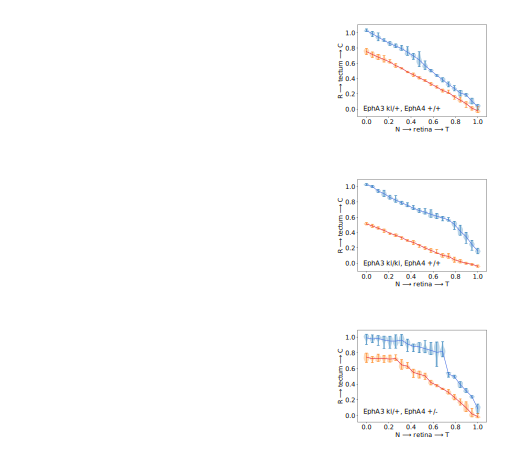
\includegraphics[width=\linewidth]{./images/EphA_manipulations.png}
\caption{Three genetic manipulations applied to the receptor-ligand model simulating those performed by \citet{brown_topographic_2000} and \citet{reber_relative_2004}. In each manipulation, the left graph shows axon branch agents (colour coded by retinal origin) at the end of a simulation ($t=1500$), the centre graph shows corresponding axon centroids, with the colour blue indicating axons with no selective manipulation and red indicating those axons with a selective genetic knock-in of EphA3. In the right hand graph, the final tectal rostro-caudal locations of axons from each naso-temporal origin in the retina are plotted as violin plots (bars indicate the max/min datum in each group and shading indicates the data distribution). Inset graphs show experimental results from  \citet{brown_topographic_2000} and \citet{reber_relative_2004}. \textbf{A} We simulated the heterozygous EphA3 knock-in (EphA3 ki/+) of \citet{brown_topographic_2000} by selecting half of the retinal cells at random, and in these cells adding the value 0.8 to $r_0$ (which, as its expression increases towards the temporal retina, is our analogue for EphA). The affected cells experienced altered interaction with tectal ligand gradients and were shifted rostrally. The rostral shift was largest for nasal cells bound for the caudal tectum. These experience the strongest interaction with $L_0$ (which is highest in caudal tectum). Temporal cells with the manipulation experience a smaller change in their final location because $L_0$ expression is low at their target location (thus the $r_0$-$L_0$ interaction is minimal). However, there is no evidence of the observed map collapse at around 0.8 on the N--T axis, as seen in the inset graph. \textbf{B} To increase the magnitude of the manipulation of EphA3, \citet{brown_topographic_2000} added a homozygous EphA3 knock-in (modelled as a knock-in of 3.2) which pushed manipulated cells further towards the rostral tectum. Here, we observed a separation into two maps, one for the wildtype cells and one for the manipulated cells, in agreement with \citet{brown_topographic_2000} (inset is from their Fig.\,5C). \textbf{C} Simulation of EphA3 ki/+ selective knock-in and EphA4 knock-down (all cells) from \citet{reber_relative_2004}. The knock-down was applied by reducing $r_0$ in all cells by 1.2. The system fails to reproduce either the map collapse at around 0.9 on the N--T axis, nor the strong rostral pull for selective knock-in cells seen in experiments. Instead, selective knock-in cells are drawn in the \emph{caudal} direction, because the knock-down of 1.2 undoes the effect of the knock-in.}
\label{f:GJeph}
\end{figure}

% FIGURE 6
\begin{figure}
\includegraphics[width=\linewidth]{./images/EphA_manipulations_explanation.png}
%% Not two mechanisms as the story. Story is that Fig 5 is ok, but not ace,
%% and we have the flexibility to propose mechanisms that fix.
\caption{Two new mechanisms to account for the genetic manipulation results: cluster-size and $r_2$ collapse. To account for map collapse (\citet{brown_topographic_2000} and Fig.\,\ref{f:GJeph}A), and for the significant rostral termination of knock-in/knock-down cells (\citet{reber_relative_2004} and Fig.\,\ref{f:GJeph}C), we assumed that i) retinal EphA interactions with tectal ephrinA ligands are modulated by EphA4 receptors through a `side-binding' mechanism and ii) EphA3 and EphA4 receptors interact with the receptors which mediate the chemotaxis effect that \emph{opposes} EphA (i.e.~with $r_2$).
\textbf{A} \emph{EphA/ephrinA expression.} As described in the text, EphA ($r_0 \equiv \sum_{i\neq 4}\mathrm{EphA}i$) is expressed according to $r_0 = 1.05 + 0.26 \exp(2.3 u)$ (green curve) where $u$ is the N--T retinal position. Knock-in is simulated by adding 0.8 to this function (giving the purple curve). Retinal ephrinA expression is a reversed version of EphA expression (green dotted curve). A threshold, $h_0$, used by the $r_2$ collapse mechanism is shown as a red dotted line, with a green dash-dot line indicating the intersection of $\Sigma\mathrm{EphA}$ and $h_0$.
\textbf{B} \emph{EphA4 expression.} Overall EphA4 expression across the retina is constant (green dotted line, value 3.5) but retinal ephrinA ($l_0$) can bind to EphA4 ($r_{A4}$), modelled here as a multiplicative interaction to give cis-bound EphA4, $r_{A4}^{\mathrm{cis}} = w_{A4} \times r_{A4} \times l_0$ (green dashed curve), where $w_{A4}$ is a binding weight described in the text. The remaining, un-bound, free EphA4 receptors, $r_{A4}^{\mathrm{free}} = r_{A4} - r_{A4}^{\mathrm{cis}}$ (green solid curve). We model genetic knock-down of EphA4 by subtracting 2.1 from $r_{A4}$, then recomputing $r_{A4}^{\mathrm{cis}}$ and $r_{A4}^{\mathrm{free}}$ to give the cyan curves.
\textbf{C} \emph{Cluster size affects signal strength.} The signal strength, $s_0$, for an interaction between EphA receptors and a tectal ligand gradient is modelled as $s_0 = r_0 \times c_0$ where $c_0$, the cluster size, is $1/r_{A4}^{\mathrm{free}}$. Shown for wildtype, knock-in and knock-down experiments, the cluster-size modulated signal $s_0$ increases for knock-in and for knock-down manipulations and is further enhanced by combined knock-in and knock-down. This cluster size-modulated signal, $s_0$, is smaller in magnitude than the signal for $r_0$ in the original model (for which $s_0 \equiv r_0$). To compensate, $r_2$ is divided by 2, which gives the correct behaviour in a wildtype system.
\textbf{D} \emph{$r_2$ collapse.} i) We assume that the strength of receptor interactions for $r_2$ collapses under the conditions that $r_0$ exceeds a threshold $h_0=2$ (red dotted line in A) and that $r_{A4}^{\mathrm{free}}$ is simultaneously below a threshold $h_{A4}=1.1626$ (red dotted line in B). Under these conditions, $r_2$ is reduced to one fifth of the value it would otherwise take. ii) The regions of $r_2$ collapse are illustrated. No collapse occurs for wildtype EphA and EphA4 expressions; in cells with only EphA4 knock-down, $r_2$ collapse occurs for temporal cells (those more temporal than the dash-dot line in A). In cells with both EphA3 knock-in and EphA4 knock-down, the collapse mechanism occurs regardless of retinal origin.}
\label{f:clustermech}
\end{figure}

% FIGURE 7
\begin{figure}
\includegraphics[width=\linewidth]{./images/EphA_manipulations_clustertheory_r2collapse.png}
\caption{Model results with the mechanisms described in Fig.\,\ref{f:clustermech}.
\textbf{A} EphA3 knock-in result for ki=0.8. The graph appears similar to that in Fig.\,\ref{f:GJeph}A but crucially, the distributions of tectal locations begin to overlap at about 80\% of the N--T axis, in agreement with experiment (inset). This is caused by the cluster size effect, in which the signal increase due to the knock-in is reduced for temporal RGCs compared with nasal cells (See Fig.\,\ref{f:clustermech}C, green/purple solid curves).
%FOR TEXT: It is confirmed by an increased achieved significance level (ASL) from a bootstrapped, studentized t-test comparing the red and blue distributions at each N--T location.
\textbf{B} The cluster size effect does not change the double knock-in result, which shows excellent agreement with experiment (inset).
\textbf{C} When EphA is knocked in and EphA4 is simultaneously knocked down, cells on the red curve experience a combination of interactions: First, the increased interaction with ephrinA that gave the result in A is still in effect. Second, all cells on the red curve experience $r_2$ collapse, whereas only temporal RGCs on the blue curve experience this effect. $r_2$ receptors are more numerous on nasal RGCs and so the collapse in $r_2$ generates a substantial rostral movement of the red curve, in agreement with \citet{reber_relative_2004}.
\textbf{D} Uniform knock-down of EphA4 in all cells (with no manipulation of EphA3) does not perturb the mapping to a significant extent, although the effect of the EphA4 knock-down on the cluster size mechanism causes a slight rostral shift in all cells.}
\label{f:r2collapse}
\end{figure}

% ANY SUPPLEMENTARY FIGURES GO AFTER THIS
%\renewcommand{\thefigure}{S\arabic{figure}}
%\setcounter{figure}{0}

% FIGURE S1
\begin{figure}
\begin{fullwidth}
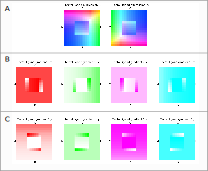
\includegraphics[width=0.95\linewidth]{./images/Tissuevisb.png}
\caption{(Supplementary) Visualisation of ligand expression and gradients on the simulated, square tectum for the
graft-rotate 90 degrees surgical manipulations.
\textbf{A} Ligand expression.
The expression of four ligand types, $L_i$,  $i = 0$--$3$, is visualised with two duochrome maps.
The lefthand map shows values for ligands $L_0$ and $L_1$ with red saturation indicating the $L_0$ expression value and green indicating the expression of $L_1$.
Elements which have high expression of both $L_0$ and $L_1$ are coloured yellow; those with expression of neither are black. The $8\times8$ square in the centre of the
The righthand map shows values for $L_2$ and $L_3$, using magenta and cyan, respectively.
\textbf{B} Visualisations of the $x$ components of the ligand gradients computed from the maps in A.
For each ligand $L_i$, the gradient $\nabla_x(L_i)$ is shown (where $x$ indicates the M--L axis).
The $x$ gradient is computed discretely as the mean difference between expression values in the neighbouring elements along the $x$ axis.
Full saturation indicates a positive gradient; white indicates a negative gradient.
For the surrounding, non-graft tissue, only the $L_1$ (green) and $L_3$ (cyan) $x$ gradients vary along the M--L axis.
Strong discontinuities in $\nabla_x$ are seen on the medial and lateral edges of the patch.
\textbf{C} Corresponding visualisations of $\nabla_y(L_i)$, with strong discontinuities in this gradient along the caudal and rostral edges of the square graft.}
\label{f:trot90}
\end{fullwidth}
\end{figure}

% FIGURE S2
\begin{figure}
\begin{fullwidth}
\includegraphics[width=0.95\linewidth]{./images/expression_profiles_EphBs.png}
\caption{(Supplementary) EphB and ephrin B gene expression.
Here, we used Stalefish \citep{james_comparing_2022} to quantitatively analyse gene expression of EphB2 and ephrinB1/B2 from images published in the literature.
\textbf{A} Retinal expression of EphB2.
We analysed Fig.\,7 of \citet{holash_polarized_1995} using `dual curves' to delineate the expression region in the Stalefish application.
The resulting, normalized expression is shown in the graph for the E4 data, with an inset showing corresponding data for the E6 data.
In the right-hand graph, we show an expansion of a portion of the E4 data to which we applied a linear fit to determine the RMS deviation from the mean to estimate the noise in the receptor signal.
The mean RMS error was 0.06.
\textbf{B} Stalefish screenshots and expression graphs for retinal ephrinB1 and ephrinB2 expression, using data from Fig.\,1 of \citet{braisted_graded_1997}.
\textbf{C} Screenshots and expression graphs for tectal ephrinB1 expression, using data from Fig.\,4 of \citet{braisted_graded_1997}.}
\label{f:expr_ephb}
\end{fullwidth}
\end{figure}

% FIGURE S3
\begin{figure}
\begin{fullwidth}
\includegraphics[width=0.95\linewidth]{./images/noise_contribution.png}
\caption{(Supplementary) Response of the model to noise.
\textbf{A} Adding 3\% gradient measurement noise (normally distributed, standard deviation, $\sigma = 0.19$) has negligible effect on the pattern.
\textbf{B} 3\% retinal receptor noise ($\sigma = 0.08$).
\textbf{C} 3\% tectal ligand noise ($\sigma = 0.08$).
\textbf{D} Combined effect of retinal receptor, tectal ligand and gradient measurement noise is dominated by the tectal ligand noise.}
\label{f:noise}
\end{fullwidth}
\end{figure}

\end{document}
